\documentclass[../main.tex]{subfiles}

\begin{document}
    Różne standardy (czyli brak standardu):
    \begin{itemize}
        \item CommonJS - serwery, Node
        \item AMD (Asynchronous Module Defintion) - przeglądarki
        \item ES2015 - wbudowane w język, ale jeszcze niezbyt rozpowszechnione
    \end{itemize}

    Moduły umożliwiają
    \begin{itemize}
        \item podział kodu na (bardziej) niezależne części
        \item łatwiejsze współdzielenie i powtórne wykorzystanie kodu
        \item ukrycie implmentacji i udostęnienie jedynie wybranych funkcji i zmiennych (interfejs)
        \item unikanie konfliktów nazw
    \end{itemize}

    \subsection{CommonJS}
    \begin{itemize}
        \item Plik modułu eksportuje funkcje i obiekty poprzez przypisując je do obiektu module.exports.
        \item Plik wykorzystujący moduł ładuje go przy pomocy funkcji require().
    \end{itemize}

    \subsection{Express.JS}
    Cechy
    \begin{itemize}
        \item Najpopularniejszy framework w Node
        \item Unopinionated - nie narzuca rozwiązań i struktury. Daje możliwość wyboru.
        \item Podpinanie obsługi pod różne metody HTTP i adresy (routing)
        \item Integracja z różnymi silnikami szablonów stron WWW
        \item Możliwość rozszerzania funkcjonalności za pomocą middleware: (obsługa sesji, cookies, logowania użytkowników, itp.)
        \item Funkcjonalność Expressa jest oparta na pojęciu middleware.
    \end{itemize}

    \textbf{Routing}
    \begin{itemize}
        \item Definiowanie obsługi dla poszczególnych metod i ścieżek: app.get(), app.post(), app.put(), app.delete() itp.
        \item Definiowanie obsługi dla dowolnej metody: app.all().
    \end{itemize}
    express.Router daje możliwość podzielenia obsługi serwisu/aplikacji webowej na części w zależności od prefiksu użytej ścieżki.
    Można dodatkowo delegować tę obsługe dododatkowego modułu. Routingi zdefinowane w express\_router.js będą dostępne w pod adresem /express\_router/ oraz /express\_router/about.

    \textbf{Ścieżki} używane przy routingu mogą być definiowane jako napisy z wzorcami, np:
    \begin{itemize}
        \item app.get('/ab?cd', callback) - '/abcd' lub '/acd'
        \item app.get('/ab+cd', callback) - '/abcd', '/abbcd', '/abbbcd', ...
        \item app.get('/ab*cd', callback) - '/abcd', '/abXcd', , '/abDowolnyTekstcd'
        \item app.get(/.*info\$/, callback)
    \end{itemize}

    \subsubsection{Model MVC (Model-View-Controller)}
    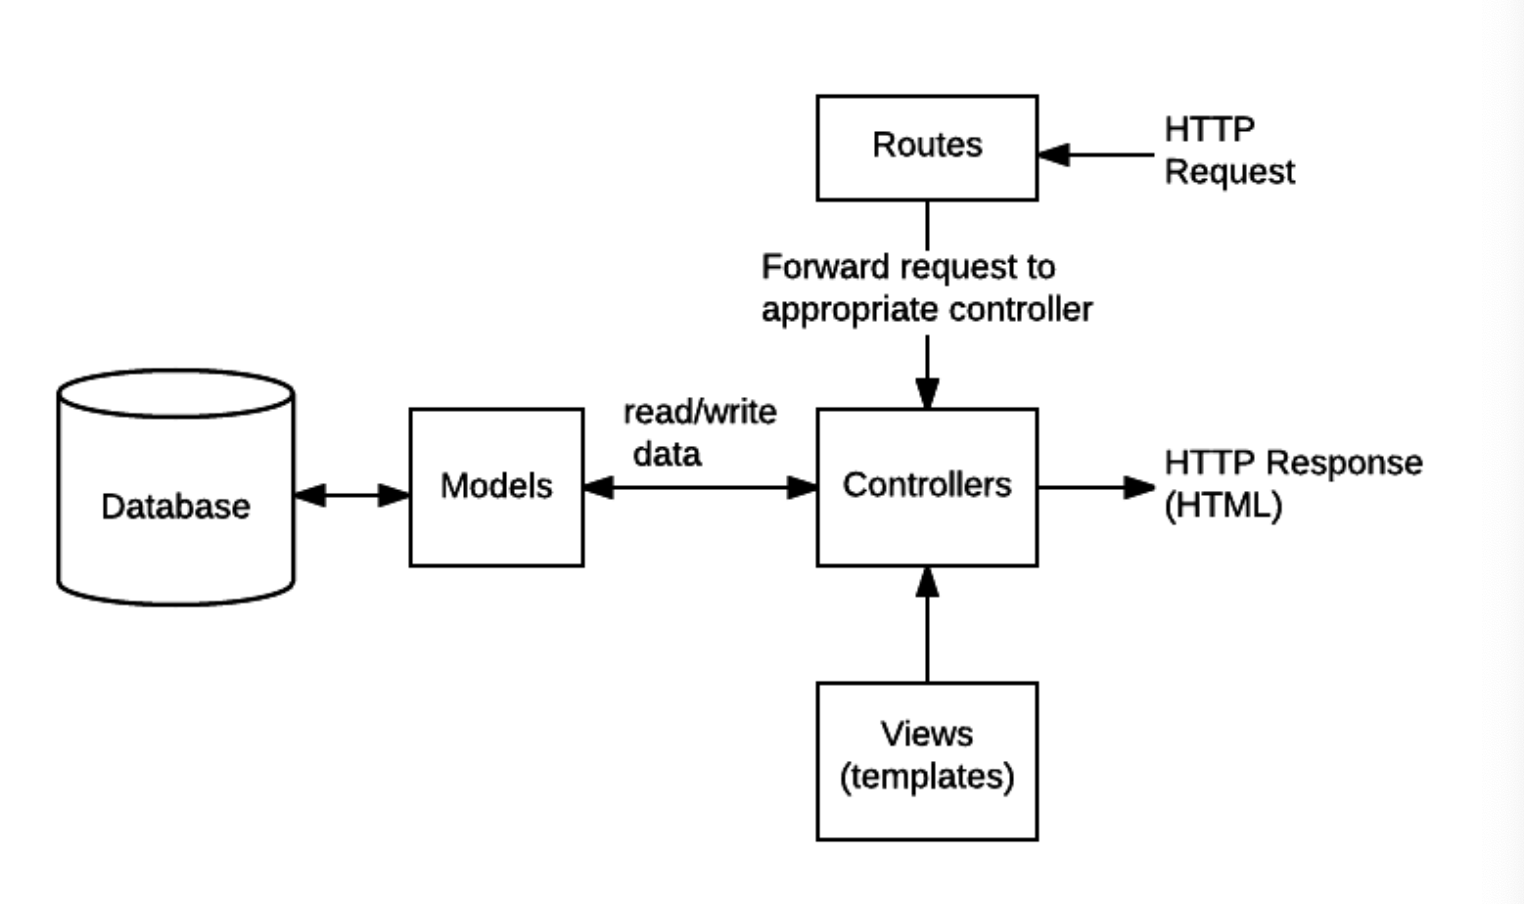
\includegraphics[width=\linewidth]{mvc.png}

    \subsection{Szablony}
    Express może współpracować z różnymi systemami szablonów HTML. Między innymi Pug, Mustache, EJS.

    \textbf{Pug}
    \begin{itemize}
        \item Zawieranie się elementów jest odzwierciedlone przy pomocy wcięć.
        \item Każda (prawie) linia zaczyna się od nazwy znacznika HTML
        \item Jeśli tag kończy się znakiem =, to dalsza częśc jest traktowana jako wyrażenie Javascript, którego wartość jest wstawiana jako zawartość generowanego elementu.
        \item Można używać instrukcji warunkowych i pętli
        \item Można również dziedziczyć/rozszrzać szablony: polecenia extend i block.
        \item Wygląda jak bardzo uproszczony html, bez nawiasów ostrych <>.
    \end{itemize}


\end{document}